%\section{Commonsense Knowledge Types}

%TODO An approach to Commonsense Knowledge Types ; explain their approach in more details there and the Reasoning ALgorithm ; explain that the Algorithm does not work as they say in the paper; the RA doesn't even the rule about the type in order to reason correctly; when I comment out ht hard coded it doesn't work
Intrigued by the remarkably achieved accuracy of the Sharma and Baral \cite{2018CommonsenseKT} approach, we now describe this work in more details. In the previous chapter, in section \ref{section:TheDifferentApproaches} we outlined \ref{Steps} of the approach. Here, we first focus on the process of identification of the presented commonsense knowledge types. Then, we discuss the proposed reasoning algorithm together with the worked out example. Finally, we give our observations and comments about this approach.


\section{Identification of Commonsense Knowledge Types}
The first step of the Sharma and Baral \cite{2018CommonsenseKT} approach is to represent the input Winograd sentence and question as semantic graphs. To achieve this, the KParser from \cite{DBLP:conf/ijcai/SharmaVAB15} is used. 
To illustrate the results of the semantic parsing, we now analyze the graphs for the sentence and question from \ref{ex:Graph} which are shown in Figure \ref{Graph11} and Figure \ref{Graph12}. \\ 
\labeltext{\textit{Example 3.1.1}}{ex:Graph}
\begin{itemize}
	\item[\textbf{S:}] \textbf{The man could not lift his son because he was weak.}
	\item[\textbf{Q:}] \textbf{Who was weak?}
\end{itemize}

In these graphs, the different colors of the nodes indicate the predefined class of nodes to which they belong. 
Nodes with red color represent events which correspond to the verbs in the sentence. Nodes with blue color represent entities and qualities of entities, and the nodes with gray color represent conceptual classes. The labels on the directed edges are the semantic relations between the different nodes in the graph. The number next to a word refers to the position of the word in the sentence. 
\begin{figure}
	\centering
	%\documentclass[border=10pt]{standalone}
%\usepackage{tikz}
\tikzset{
	treenode/.style = {shape=rectangle, rounded corners,
		draw, align=center,
		top color=white, bottom color=blue!20},
	root/.style     = {treenode, font=\ttfamily\normalsize},
	env/.style      = {treenode, font=\ttfamily\normalsize},
	dummy/.style    = {circle,draw},
	level 1/.style={sibling distance=8cm, level distance = 3em, label = 1pt },
	level 2/.style={sibling distance=2.5cm,level distance = 5em}, 
	level 3/.style={sibling distance=2cm},
	blueRed/.style={env, top color=blue, bottom color=red} 
}
%\begin{document}

	\begin{tikzpicture}
	[
	grow                    = down,
	sibling distance        = 50em,
	level distance          = 5em,
	edge from parent/.style = {draw, -latex},
	every node/.style       = {font=\footnotesize},
	sloped
	]
	\node [root] {\underline{was-10}}
	child { node [env] {\textbf{he-9}}
	  child {node [env] {\textbf{weak-11}}
	  	 child {node [env] {\textit{weak}}
	  		child {node [env] {\textit{quality}}
	  			edge from parent node [below] {subclass}}
	  		edge from parent node [below] {inst\_of}}
			edge from parent node [above] {trait}}
	  child {node [env] {\textit{he}}
	  		child {node [env] {\textit{person}}
	  			edge from parent node [below] {subclass}}
	  		edge from parent node [above] {inst\_of}}	
	   edge from parent node [above] {agent}}
	child { node [env] {\underline{lift-5}}
	  child {node [env]  {\textbf{could-3}}
	  	edge from parent node [above] {modal\_verb} }	
	  child {node [env]  {\textbf{man-2}}
	  	child {node [env] {\textit{man}}
	  		 child {node [env] {\textit{person}}
	  			edge from parent node [below] {subclass}}
	  		edge from parent node [below] {inst\_of}}
	  	edge from parent node [above] {agent} }
	  child {node [env]  {\textbf{son-7}}
	  	child {node [env] {\textbf{his-6}}
	  		child {node [env] {\textit{his}}
 			  	child {node [env] {\textit{person}}
  				   edge from parent node [below] {subclass}}
	  			edge from parent node [below] {inst\_of}}
	  		edge from parent node [above] {relate\_to}}
  		child {node [env] (son) {\textit{son}}
  			child {node [env] {\textit{person}}
  				edge from parent node [above] {subclass}}
  		 edge from parent node [above] {inst\_of}}
	  	edge from parent node [above] {recipient}}
	  child {node [env]  {\textbf{not-4}}
			edge from parent node [above] {negation} }
	 child {node [env] [right=8mm of son]  {\textit{lift}}
			edge from parent node [below] {inst\_of} }
		edge from parent node [above] {cause}};
	

	\end{tikzpicture}
%\end{document}
	\caption{\label{Graph11}``The man couldn't lift his son because he was so weak."}
\end{figure}


\begin{figure}
	\centering
	%\documentclass[border=10pt]{standalone}
%\usepackage{tikz}
\tikzset{
	treenode/.style = {shape=rectangle, rounded corners,
		draw, align=center,
		top color=white, bottom color=blue!20},
	root/.style     = {treenode, font=\ttfamily\normalsize, bottom color=red!30},
	env/.style      = {treenode, font=\ttfamily\normalsize},
	dummy/.style    = {circle,draw},
	level 1/.style={sibling distance=3cm, level distance = 3em},
	level 2/.style={sibling distance=1.7cm,level distance = 5em}, 
	level 3/.style={sibling distance=2cm},
	blueRed/.style={env, top color=blue, bottom color=red} 
}
%\begin{document}
\begin{tikzpicture}
[
grow                    = down,
sibling distance        = 50em,
level distance          = 5em,
edge from parent/.style = {draw, -latex},
every node/.style       = {font=\footnotesize},
sloped
]
\node [root] {weak-3}
	child {node [env] {person}
		edge from parent node [above] {inst\_of}}
	child {node [env] {q}
		edge from parent node [above] {inst\_of}} 	
	edge from parent node [above] {trait\_of}}
child {node [env] {weak}
		edge from parent node[above] {inst\_of}};


\end{tikzpicture}
%\end{document}
	\caption{\label{Graph12}``Who was weak?"}
\end{figure}

For the representation of the question, one additional conceptual class labeled as "q" is introduced. In this conceptual class are all nodes which represent the question words from the WSC problems, such as: \textit{Who, Which and What}.

From the observation of these two graphs, Sharma and Baral \cite{2018CommonsenseKT} come to conclusion that the missing knowledge required in order to answer the question, must connect the trait of an entity being weak with its inability to lift. In Figure 3 is the representation of this knowledge as shown in \cite{2018CommonsenseKT}. 

%TODO add here graph for their type
\begin{comment}
	content...

\begin{figure}
	\centering
	%\documentclass[border=10pt]{standalone}
%\usepackage{tikz}
\tikzset{
	treenode/.style = {shape=rectangle, rounded corners,
		draw, align=center,
		top color=white, bottom color=blue!20},
	root/.style     = {treenode, font=\ttfamily\normalsize},
	env/.style      = {treenode, font=\ttfamily\normalsize},
	dummy/.style    = {circle,draw},
	level 1/.style={sibling distance=6cm, level distance = 1em},
	level 2/.style={sibling distance=2.5cm,level distance = 5em}, 
	level 3/.style={sibling distance=2cm},
	blueRed/.style={env, top color=blue, bottom color=red} 
}
%\begin{document}
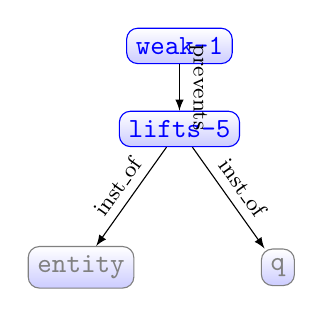
\begin{tikzpicture}
[
grow                    = down,
sibling distance        = 50em,
level distance          = 5em,
edge from parent/.style = {draw, -latex},
every node/.style       = {font=\footnotesize},
sloped
]
\node  [env, blue] {weak-1}
child { node [env, blue] {lifts-5}
	child {node [env, gray] {entity}
		edge from parent node [above] {inst\_of}}
	child {node [env, gray] {q}
		edge from parent node [above] {inst\_of}} 	
	edge from parent node [above] {prevents}};


\end{tikzpicture}
%\end{document}
	\caption{\label{Graph13}``Prevents type?"}
\end{figure}
\end{comment}

By applying this observation to all problems from the WSC corpus, Sharma and Baral \cite{2018CommonsenseKT} identified 12 different knowledge types. From these, the first 10 knowledge types share the same structure as they are all based on different interactions between actions and properties. Each of the 10 knowledge types consists of three parts: the first and third part are sentences containing entities, properties or actions, whereas the second part is a semantic relation (\textit{causes, prevents} or \textit{followed by}) which connects them. The last two knowledge types have different structure because one of them requires multiple knowledge and the other one is based on the conditional likelihood of a previous event. 
For the representation of the knowledge type shown in Figure 1.3, the first part is \textit{weak y}, the third part is \textit{y lifts} and the semantic relation is \textit{prevents}.
The presented identified knowledge types are the following:

\begin{quote} 
	Property \textit{prevents} Action, Action1 \textit{prevents} Action2, Action1 \textit{causes} Action2, Property \textit{causes} Action, Action \textit{causes} Property, Property1 \textit{causes} Property2, Action1 \textit{followed by} Action2, Action \textit{followed by} Property, Property \textit{followed by} Action, Co-existing Action(s) and Property(s), Statement1 \textit{is more likely than} Statement2, Multiple Knowledge. 
\end{quote}


\section{Reasoning Algorithm}
We will now explain the proposed Reasoning Algorithm (RA) which was used for answering the WSC problems by using the previously explained knowledge types. The RA together with a running example is available online\footnote{https://drive.google.com/file/d/1WN0T98HaMFhWEEIH-3AlWoIPxAdFYlT\_/view}. The code for the RA algorithm can be found in Appendix\ref{AppendixA}. 

%TODO clarify cross domain sibling vs clone

The RA is based on Answer Set Programming (ASP) \cite{DBLP:conf/aaai/Lifschitz08}. 
The RA is split into two phases, each including several steps. Each step, results in creating new ASP rules.
In the second phase, the graph representation of the WSs question is matched with the merged representation from the first phase. With this matching, the possible answer should be retrieved. 
\begin{itemize}
	\item \textbf{Phase 1: Generating merged representation}\\
	 In this phase, the graph representation of the Winograd sentence and the background knowledge are analyzed and the following information from both is extracted and merged.
	\begin{enumerate}
		\item All the nodes which are an instance of a defined class of nodes (for example: person, motion, description) in the KParser are identified as constant nodes. 
		\item Nodes with parents as constant nodes are identified. 
		\item Nodes with children as constant nodes are identified. 
		\item The cross domain siblings in both representations are identified. These are constant nodes which appear in both graphs and they both are instances of nodes of the same type. Furthermore the cross domain siblings ave the same number of child/parent nodes which are connected through the same semantic relations. 
		\item A merged representation is generated
		
	\end{enumerate}
	\item \textbf{Phase 2: Extracting possible answers}\\
	In this phase, the graph representation of the WSs question is projected on the merged representation from the previous step. The goal is to retrieve the nodes which are cross domain clones of the unknown nodes (q)  in the graph representation of the question.
	\begin{enumerate}
		\item Constant nodes are identified from both graphs.
		\item Nodes with children/parent as constant node are identified. 
		\item Cross domain siblings of the nodes from the question graph are identified.
		\item Using the previous nodes, the cross domain clones of the nodes from the question graph are identified. 
	\end{enumerate}
\end{itemize}


The reasoning algorithm can reason over 10 of the 12 identified categories.

\section{Observations}
%TODO add this to discussion; not here
The encoding the example available in the supplementary document resulted in correct answer. 
After that we tried a few different sentences and the reasoning algorithm worked correctly. 
When the rule that defines the knowledge type is commented out, again a correct answer is retrieved. 
Our conclusion is that the RA does not even use this rule in the reasoning process. Rather it relies on hard coded information about the agent and the recipient of the action.